\documentclass[sigplan, anonymous, review]{acmart}

\usepackage{booktabs} % For formal tables


% Copyright
%\setcopyright{none}
%\setcopyright{acmcopyright}
%\setcopyright{acmlicensed}
\setcopyright{rightsretained}
%\setcopyright{usgov}
%\setcopyright{usgovmixed}
%\setcopyright{cagov}
%\setcopyright{cagovmixed}


% DOI
\acmDOI{10.475/123_4}

% ISBN
\acmISBN{123-4567-24-567/08/06}

%Conference
\acmConference[WOODSTOCK'97]{ACM Woodstock conference}{July 1997}{El
  Paso, Texas USA}
\acmYear{1997}
\copyrightyear{2016}

\acmPrice{15.00}

%\acmBadgeL[http://ctuning.org/ae/ppopp2016.html]{ae-logo}
%\acmBadgeR[http://ctuning.org/ae/ppopp2016.html]{ae-logo}


\begin{document}
\title{SIG Proceedings Paper in LaTeX Format}
\titlenote{Produces the permission block, and
  copyright information}
\subtitle{Extended Abstract}
\subtitlenote{The full version of the author's guide is available as
  \texttt{acmart.pdf} document}

\author{Ben Trovato}
\authornote{Dr.~Trovato insisted his name be first.}
\orcid{1234-5678-9012}
\affiliation{%
  \institution{Institute for Clarity in Documentation}
  \streetaddress{P.O. Box 1212}
  \city{Dublin}
  \state{Ohio}
  \postcode{43017-6221}
}
\email{trovato@corporation.com}

\author{G.K.M. Tobin}
\authornote{The secretary disavows any knowledge of this author's actions.}
\affiliation{%
  \institution{Institute for Clarity in Documentation}
  \streetaddress{P.O. Box 1212}
  \city{Dublin}
  \state{Ohio}
  \postcode{43017-6221}
}
\email{webmaster@marysville-ohio.com}

\author{Lars Th{\o}rv{\"a}ld}
\authornote{This author is the
  one who did all the really hard work.}
\affiliation{%
  \institution{The Th{\o}rv{\"a}ld Group}
  \streetaddress{1 Th{\o}rv{\"a}ld Circle}
  \city{Hekla}
  \country{Iceland}}
\email{larst@affiliation.org}

\author{Valerie B\'eranger}
\affiliation{%
  \institution{Inria Paris-Rocquencourt}
  \city{Rocquencourt}
  \country{France}
}
\author{Aparna Patel}
\affiliation{%
 \institution{Rajiv Gandhi University}
 \streetaddress{Rono-Hills}
 \city{Doimukh}
 \state{Arunachal Pradesh}
 \country{India}}
\author{Huifen Chan}
\affiliation{%
  \institution{Tsinghua University}
  \streetaddress{30 Shuangqing Rd}
  \city{Haidian Qu}
  \state{Beijing Shi}
  \country{China}}

\author{Charles Palmer}
\affiliation{%
  \institution{Palmer Research Laboratories}
  \streetaddress{8600 Datapoint Drive}
  \city{San Antonio}
  \state{Texas}
  \postcode{78229}}
\email{cpalmer@prl.com}

\author{John Smith}
\affiliation{\institution{The Th{\o}rv{\"a}ld Group}}
\email{jsmith@affiliation.org}

\author{Julius P.~Kumquat}
\affiliation{\institution{The Kumquat Consortium}}
\email{jpkumquat@consortium.net}


% The default list of authors is too long for headers.
\renewcommand{\shortauthors}{B. Trovato et al.}


\begin{abstract}
This paper provides a sample of a \LaTeX\ document which conforms,
somewhat loosely, to the formatting guidelines for
ACM SIG Proceedings.
\end{abstract}

%
% The code below should be generated by the tool at
% http://dl.acm.org/ccs.cfm
% Please copy and paste the code instead of the example below.
%
\begin{CCSXML}
<ccs2012>
 <concept>
  <concept_id>10010520.10010553.10010562</concept_id>
  <concept_desc>Computer systems organization~Embedded systems</concept_desc>
  <concept_significance>500</concept_significance>
 </concept>
 <concept>
  <concept_id>10010520.10010575.10010755</concept_id>
  <concept_desc>Computer systems organization~Redundancy</concept_desc>
  <concept_significance>300</concept_significance>
 </concept>
 <concept>
  <concept_id>10010520.10010553.10010554</concept_id>
  <concept_desc>Computer systems organization~Robotics</concept_desc>
  <concept_significance>100</concept_significance>
 </concept>
 <concept>
  <concept_id>10003033.10003083.10003095</concept_id>
  <concept_desc>Networks~Network reliability</concept_desc>
  <concept_significance>100</concept_significance>
 </concept>
</ccs2012>
\end{CCSXML}

\ccsdesc[500]{Computer systems organization~Embedded systems}
\ccsdesc[300]{Computer systems organization~Redundancy}
\ccsdesc{Computer systems organization~Robotics}
\ccsdesc[100]{Networks~Network reliability}


\keywords{ACM proceedings, \LaTeX, text tagging}

\begin{teaserfigure}
  %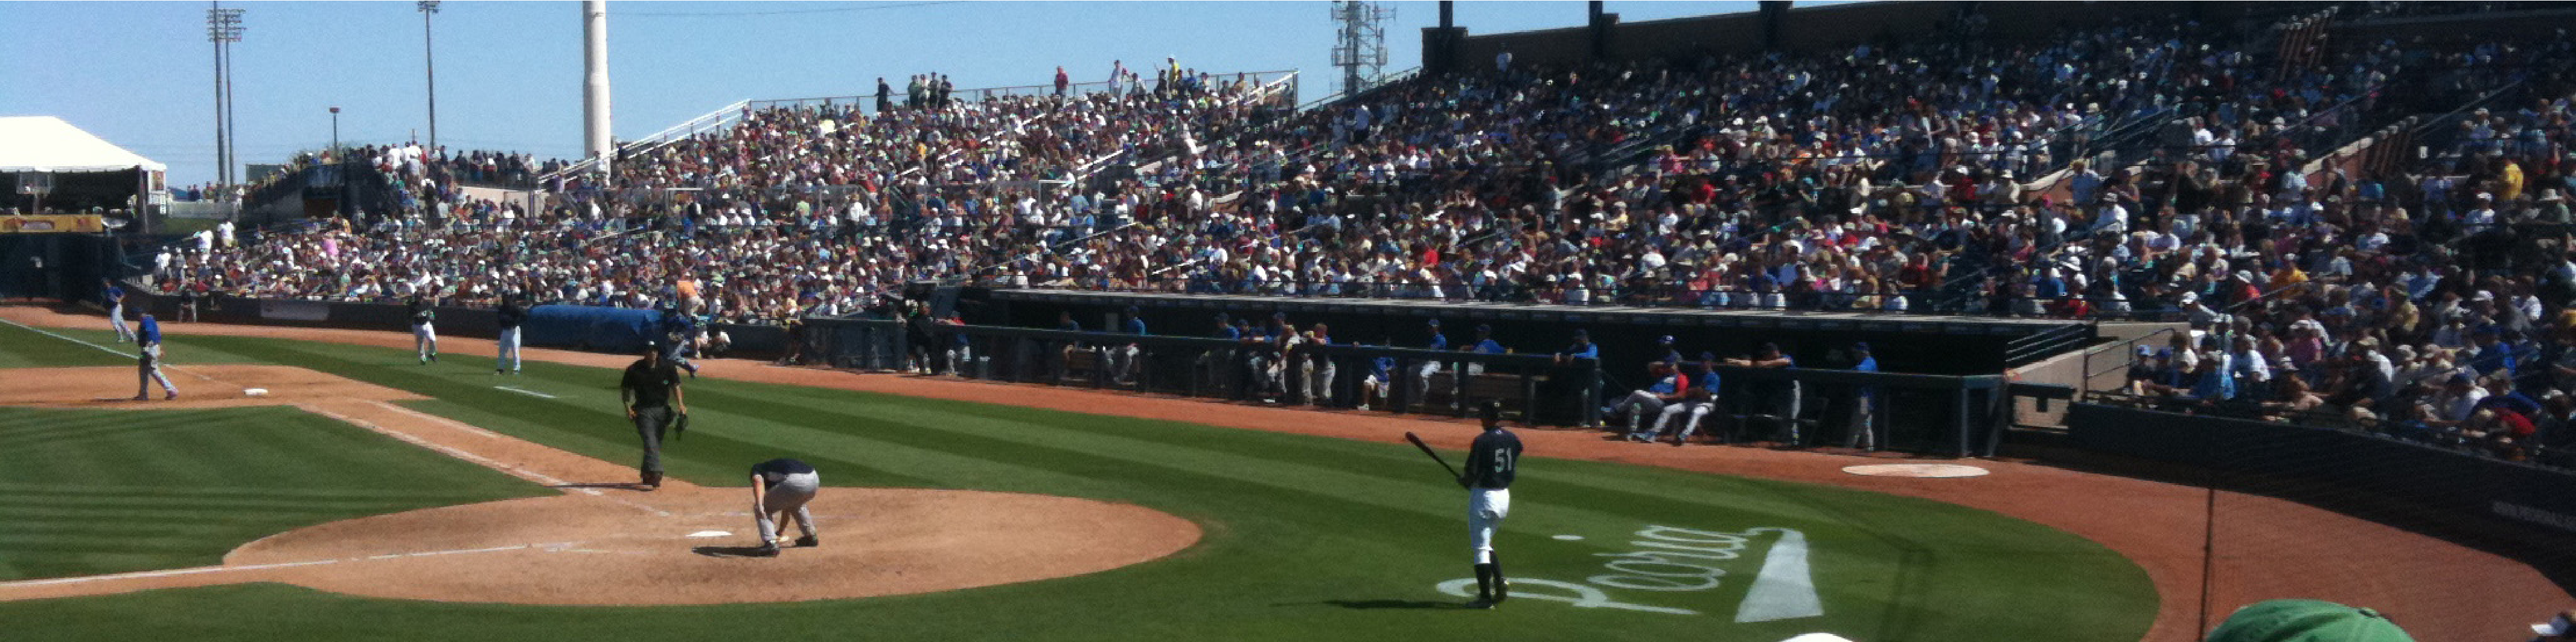
\includegraphics[width=\textwidth]{sampleteaser}
  \caption{This is a teaser}
  \label{fig:teaser}
\end{teaserfigure}


\maketitle

\label{sec.introduction}

According to the International Energy Agency (IEA), the number of
network-connected devices is expected to reach 50 billion by 2020 with the
expansion of the Internet of Things (IoT)~\cite{iea.data}.
%
However, most of the energy to power these devices will be consumed in
\emph{standby mode}, i.e., when they are neither transmitting or processing
data.
%
For instance, standby power currently accounts for approximately 10--15\% of
residential electricity consumption, and $CO_2$ emissions related to standby
are equivalent to those of 1 million cars~\cite{iea.data,standby.australia}.
%
The projected growth of IoT devices, together with the surprising effects of
standby consumption, made network standby efficiency one of the six
pillars of the \emph{G20's Energy Efficiency Action Plan}%
\footnote{G20's Energy Efficiency Action Plan: \url{https://www.iea-4e.org/projects/g20}}.
%
However, making effective use of standby requires software-related efforts in
order to detect idle periods of activity in the device, identify peripherals
that must remain functional, and apply appropriate sleep mode levels in the
microcontroller.

Given the projected scale of the IoT, the role of low-power standby towards
energy efficiency, and the posed software-related challenges, our research has
the following goals:
%
%\begin{enumerate}
(i)   address energy efficiency through meticulous use of standby;
(ii)  target low-power, resource-constrained embedded architectures that form
      the IoT;
(iii) provide standby mechanisms at the programming language level that scale
      to all applications; and
(iv)  support transparent/non-intrusive standby mechanisms that reduce barriers
      of adoption.
%\end{enumerate}

Our approach lies at the bottom of the software development
layers---programming language mechanisms---meaning that \emph{all} applications
should take advantage of low-power standby modes automatically, without extra
programming efforts.
%
We extend the programming language \CEU~\cite{ceu.sensys13,ceu.tecs17} with
support for interrupt service routines (ISRs) and with a simple power
management runtime (PMR).
%
Our approach relies on the synchronous semantics of the language which enforces
that reactions to the environment always reach an idle state amenable to
standby.

Each supported microcontroller requires bindings in C for the ISRs and PMR, and
each peripheral requires a driver in \CEU.
These are write-once code that are typically packaged and distributed in a
software development kit (SDK).
%
Then, all new applications built on top of these drivers take advantage of
standby automatically.
%
As a proof of concept, we provide an open source SDK %
%\footnote{https://github.com/fsantanna/ceu-arduino/}
with support for 8-bit
\emph{AVR/ATmega} and 32-bit \emph{ARM/Cortex-M0} microcontrollers, and a
variety of peripherals, such as for GPIO, A/D converter, USART, SPI, and the
nRF24L01 transceiver.
%
We developed a number of simple applications using these peripherals
concurrently and could verify that the applications remain in the deepest
standby modes for the longest periods of time.

In Section~\ref{sec.ceu}, we compare the structure of programs in \CEU and
Arduino~\cite{arduino.book}, whose primary goal is to reduce the barrier of
adoption for a non-technical audience (e.g., designers and artists).
We show that we can keep the intended sequential reasoning of Arduino even when
applications require non-trivial concurrent behavior.
%
In Section~\ref{sec.standby}, we discuss the software infrastructure that
allows for unmodified programs in \CEU to take advantage of standby
automatically.
%
In Section~\ref{sec.conclusion}, we discuss future work and conclude the paper.

% - standby as well as enabled/disabled, powered, switched
% - application on IoT
% - results
%   - atmega 328p/2560
%   - arm cortex-m0
%   - how much efficiency?
% - limitations

%In Section~\ref{sec.ceu}, we introduce the structured synchronous model and the
%programming language \CEU.
%In Section~\ref{sec.apps}, we evaluate .
%In Section~\ref{sec.ext}, we present the language extensions that support
%transparent standby.

\section{The Structured Synchronous Programming Language \CEU}
\label{sec.ceu}

\begin{comment}
- structured programming
- lexical scope

In summary:

Reactive: code executes in reactions to events

Synchronous: reactions run to completion, i.e., there's no implicit preemption or real parallelism (this avoids explicit synchronization: locks, queues, etc)

Structured: programs use structured control mechanisms, such as "await" (to suspend a line of execution), and "par" (to combine multiple awaiting lines of execution)

Structured programming avoids deep nesting of callbacks letting you write programs in direct/sequential style. In addition, when a line of execution is aborted, all allocated resources are safely released.

In comparison to FRP/dataflow, it is more imperative supporting sequences/loops/conditionals/parallels. The notion of (multiple) program counter is explicit. Also, everything is lexically scoped, there's no GC involved.

In comparison to promises/futures, it provides lexical parallel constructs, allowing the branches to share local variables and, more importantly, supporting safe abortion of code (with the "par/or").
\end{comment}

\CEU is a Esterel-based~\cite{ceu.tecs17} reactive programming language
targeting resource-constrained embedded systems~\cite{ceu.sensys13}.
%
It is grounded on the synchronous concurrency model, which has been
successfully adopted in the context of hard real-time systems such as avionics
and automobiles industry since the 80's~\cite{rp.twelve}.
%
The synchronous model trades power for reliability and has a simpler model
of time that suits most requirements of IoT applications.
%
On the one hand, this model cannot directly express time-consuming
computations, such as compression and cryptography algorithms, which are
typically either absent or delegated to auxiliary chips in the context of the
IoT.
%
On the other hand, all reactions to the external environment are guaranteed to
be computed in bounded time, ensuring that applications always reach an idle
state amenable to standby mode.
%
Overall, \CEU aims to offer a concurrent, safe, and expressive alternative to C
with the characteristics that follow:
%
\begin{description}
\item [Reactive:] code only executes in reactions to events and is idle most of
    the time.
\item [Structured:] programs use structured control mechanisms, such as
    \code{await} (to suspend a line of execution), and \code{par} (to combine
    multiple lines of execution).
\item [Synchronous:] reactions run atomically and to completion on each line of
    execution, i.e., there's no implicit preemption or real parallelism.
\end{description}
%
Structured reactive programming lets developers write code in direct style,
recovering from the inversion of control imposed by event-driven
execution~\cite{rp.deprecating,rp.rescala,sync_async.cooperative}.

\subsection*{A Motivating Example}
\label{sec.ceu.example}

{\linespread{1}
\begin{figure}[t]
\begin{minipage}[t]{0.49\linewidth}
\begin{lstlisting}[xrightmargin=0.5cm]
while (1) {
  delay(1000);
  int v =
    analogRead();
  radioWrite(v);
}
\end{lstlisting}
\centering\small{[a] Version in Arduino}
\end{minipage}
%
\begin{minipage}[t]{0.49\linewidth}
\begin{lstlisting}[numbers=left,xleftmargin=-0.2cm]
loop do
  await 1s;
  var int v =
    await AnalogRead();
  await RadioWrite(v);
end
\end{lstlisting}
\centering\small{[b] Version in \CEU}
\end{minipage}
%\rule{8.4cm}{0.37pt}
\caption{ Sequence of I/O operations running in a loop.
\label{lst.direct}
}
\end{figure}
}

Figure~\ref{lst.direct}.a shows a straightforward, easy-to-read code snippet
in Arduino that executes forever in a loop a sequence of operations as follows:
    waits for 1 second (ln. 2),
    performs an A/D conversion (ln. 3--4), and
    broadcasts the read value (ln. 5).
%
Figure~\ref{lst.direct}.b shows the same code in \CEU, with the noteworthy
difference that operations that interact with the environment and take time use
the \code{await} keyword. % and can be easily identified in the program.
%
The traditional structured paradigm encouraged in Arduino (with blocks, loops,
and sequences) allows for simple and readable code, avoiding the complexity of
dealing with ISRs.
%
However, the use of blocking operations, such as \code{delay(1000)} (ln. 2),
prevents that other operations execute concurrently.

Suppose that we now want to immediately abort the loop in
Figure~\ref{lst.direct}.a at any time, as soon as a radio message arrives.
%
Since the message might arrive concurrently with any of the blocking
operations, we need to change the structure of the program.
%
Figure~\ref{lst.inversion}.a changes the blocking \code{delay} to the polling
\code{millis}, which immediately returns the number of milliseconds since the
reset.
Now, we start by registering the current time (ln. 1--2) and, on each loop
iteration, we recheck the time to see if one second has elapsed (ln. 7--9).
Since these operations are non-blocking, we can intercalate their execution
with checks for message arrivals (ln. 4--6).
If the time is up, we start counting it again (ln. 10) before proceeding to the
original operations in sequence (ln. 11--13).
%
The original structured style in Figure~\ref{lst.direct}.a has been drastically
violated to accommodate concurrency in Figure~\ref{lst.inversion}.a.
In the example, we only adapted the \code{delay} operation, but the other
blocking operations (\code{analogRead} and \code{radioWrite}) would also need
to be changed to achieve maximum concurrency.
%
Alternatively, we could resort to ISRs or implement an event-driven
scheduler to handle the operations~\cite{wsn.nesc}, but ultimately, the
program readability would still be compromised.

The program in Figure~\ref{lst.inversion}.b in \CEU extends the one in
Figure~\ref{lst.direct}.b to accommodate concurrency.
%
In contrast with the Arduino version, the original code in \CEU remains
unmodified (Figure~\ref{lst.inversion}.b, ln. 4--9) and concurrency is achieved
through the \code{par/or} construct, which creates two lines of execution and
terminates when either of them terminates, aborting the other automatically.
%
This approach preserves the sequential, easy-to-read style while introducing
concurrency seamlessly.

\begin{figure}[t]
\begin{minipage}[t]{0.49\linewidth}
\begin{lstlisting}[xrightmargin=0.5cm]
uint32_t prv =
  millis();
while (1) {
  if (radioAvail()) {
    break;
  }
  uint32_t cur =
    millis();
  if (cur>prv+1000) {
    prv = cur;
    int v =
      analogRead();
    radioWrite(v);
  }
}
\end{lstlisting}
\centering\small{[a] Version in Arduino}
\end{minipage}
%
\begin{minipage}[t]{0.49\linewidth}
\begin{lstlisting}[numbers=left,xleftmargin=-0.2cm]
par/or do
  await RadioAvail();
with
  loop do
    await 1s;
    var int v =
      await AnalogRead();
    await RadioWrite(v);
  end
end




.
\end{lstlisting}
\centering\small{[b] Version in \CEU}
\end{minipage}
%\rule{8.4cm}{0.37pt}
\caption{ Achieving concurrency between I/O operations.
\label{lst.inversion}
}
\end{figure}

\subsection*{Standby Considerations}
\label{sec.ceu.standby}

The structure of the program in Figure~\ref{lst.inversion}.b also indicates
which peripherals are active at a given time.
%
For instance, when the program is awaiting concurrently in lines 2 and 7,
only the radio transceiver and A/D converter can awake the program.
Hence, the language runtime can choose the most energy-efficient sleep mode
that allows these peripherals to awake the microcontroller from associated
interrupts.
%
Since the semantics of \CEU enforces the program to always reach \code{await}
statements in all active lines of execution, it is always possible to put the
microcontroller into the optimal sleep mode after each reaction to the
environment.

\section{Standby Infrastructure}
\label{sec.standby}

In order to empower the example in Figure~\ref{lst.inversion}.b with automatic
standby, we developed some extensions to \CEU:
%
\begin{itemize}
\item We made the runtime of \CEU interrupt driven and put the microcontroller
      in standby after each reaction to the environment.
\item We provided operations for the drivers to indicate which interrupts can
      awake the program.
\item We included support for ISRs in \CEU to generate input events to the
      program.
\end{itemize}

Figure~\ref{lst.adc} shows the driver for the A/D converter in \CEU.
This code is specific to the \emph{ATmega328p} microcontroller and must be
adapted to work in other platforms.
For simplicity, we assume in the paper that the converter has a single channel
to avoid having to deal with multiplexing.

The driver exposes raw I/O events (ln. 3--4) that only deal with low-level
port manipulation in the microcontroller.
Output events are triggered with the \code{emit} keyword (ln. 29), while input
events are captured with the \code{await} keyword (ln. 30).
%
The output event \code{ADC\_REQUEST} (ln. 9--15) enables ADC interrupts and
starts an analog-to-digital conversion asynchronously in the peripheral for
the single channel \code{A0}.
In \CEU, any code in between \code{\{} and \code{\}} is treated as an inline
$C$ chunk, allowing for easy integration with $C$ for low-level operations.

The \code{async/isr} construct of \CEU defines an ISR which executes
asynchronously with the program when the specified interrupt occurs.
Only ISRs can emit input events to the program.
In the example, we define an ISR to handle \code{ADC} interrupts which fire
whenever a conversion is complete (ln. 17--21).
%
Although the ISR body executes asynchronously on interrupts, the input emission
(ln. 20) only takes effect on a subsequent reaction, when the synchronous part
of the program is idle.
%
This way, race conditions are only possible with \code{async/isr} blocks, which
are typically hidden inside device drivers.
\CEU also provides an \code{atomic} primitive to protect critical sections of
code.

The low-level events are the pieces that vary among platforms.
A driver can also expose a higher-level portable abstraction to client code.
%
In the example, the \code{AnalogRead} abstraction (ln. 23--33) takes care of
starting and awaiting the conversion (ln. 29--30), as well as dealing with the
power management runtime (PMR).
%
The \code{PM\_SET(PM\_ADC,1)} (ln. 24) tells the system that, when entering in
sleep mode, the \code{ADC} must be kept running.
%
The \code{PM\_SET(PM\_ADC,0)} inside the \code{finalize} clause (ln. 25--27)
releases the \code{ADC} subsystem from the PMR.

The \code{finalize} construct of \CEU executes the nested code whenever its
enclosing block terminates or is aborted externally.
%
The example of Figure~\ref{lst.inversion}.b invokes the \code{AnalogRead}
abstraction (ln. 7) concurrently with \code{RadioAvail} (ln. 2).
%
The \code{AnalogRead} may terminate normally or a radio message may arrive
during the A/D conversion, causing the \code{AnalogRead} to abort abruptly.
In either case, the \code{finalize} clause executes and puts the PMR in a
consistent state.

\begin{figure}[t]
\begin{lstlisting}[numbers=left]
// Exposed driver functionality

output void ADC_REQUEST; // low-level request
input  int  ADC_DONE;    // low-level response
code AnalogRead (void) -> int; // high-level abstraction

// Driver implementation

output void ADC_REQUEST do
  {
    ADMUX = 0x40 | (A0 & 0x07);
    bitSet(ADCSRA, ADIE); // enables interrupt
    bitSet(ADCSRA, ADSC); // starts the conversion
  }
end

async/isr {ADC_vect_num} do
  { bitClear(ADCSRA, ADIE); } // disables interrupt
  var int value = {ADC}; // reads register with the value
  emit ADC_DONE(value);
end

code AnalogRead (void) -> int do
  {PM_SET(PM_ADC, 1);}
  do finalize with
      {PM_SET(PM_ADC, 0);}
  end

  emit ADC_REQUEST;
  var int value = await ADC_DONE;

  escape value;
end
\end{lstlisting}
%\rule{8.4cm}{0.37pt}
\caption{ \CEU driver for the \emph{ATmega328p} A/D converter.
\label{lst.adc}
}
\end{figure}

The PMR also expects a platform-specific power management module to be able to
put the microcontroller into the most efficient sleep mode possible.
%
The code in Figure~\ref{lst.pm} implements the \code{pm\_sleep} function for
the \emph{ATmega328p} microcontroller which the PMR calls when the program is
idle.
%
Each device has an associated index (ln. 6--10) in the \code{pm} bit vector
(ln. 4).
%
The driver manipulates its device's index to indicate its state
(Figure~\ref{lst.adc}, ln. 24,26).
%
The \code{pm\_sleep} queries the vector to choose the appropriate sleep mode.
In the example, if the timer is active (ln. 13), the microcontroller can only
use the least efficient mode%
\footnote{
    We use an external library for the sleep modes:
    \url{http://www.rocketscream.com/blog/2011/07/04/lightweight-low-power-arduino-library/}
}
(ln. 14).
%
In the best case, e.g., if only external interrupts are required, the
microcontroller can use the most efficient mode (ln. 18).

With all the standby infrastructure set, the unmodified program of
Figure~\ref{lst.inversion}.b will automatically take advantage of the deepest
sleep modes for the longest periods of time possible.

\begin{figure}[t]
\begin{lstlisting}[numbers=left]
#define PM_GET(dev)   bitRead(pm,dev)
#define PM_SET(dev,v) bitWrite(pm,dev,v)

static u32 pm = 0; // up to 32 peripherals

enum {
  CEU_PM_ADC = 0,
  CEU_PM_TIMER1,
  <...>,
};

void pm_sleep (void) {
  if (PM_GET(PM_TIMER1) || <...>) {
      LowPower.idle(PM_GET(PM_ADC),<...>)
    } else if (PM_GET(PM_ADC)) {
      LowPower.adcNoiseReduction(<...>);
    } else {
      LowPower.powerDown(<...>);
    }
  }
}
\end{lstlisting}
%\rule{8.4cm}{0.37pt}
\caption{ Power management module for the \emph{ATmega328p} microcontroller.
\label{lst.pm}
}
\end{figure}

\section{Conclusion and Future Work}
\label{sec.conclusion}

In this work, we address standby efficiency for embedded devices at the level
of programming languages.
%
We propose a software infrastructure for the programming language \CEU that
encompasses a power management runtime and support for interrupt service
routines in the language.
%
Our approach relies on the synchronous semantics of the language which enforces
that reactions to the environment always reach an idle state amenable to
standby.
%
This way, application written in \CEU can take advantage of the longest periods
of time and deepest sleep modes possible without extra programming efforts.

In future work, in order to evaluate the gains in energy efficiency with the
proposed infrastructure, we will evaluate the consumption of realistic
applications.
%
The Arduino community has an abundance of open-source projects which can be
rewritten in \CEU to take advantage of transparent standby.
%
In this scenario, we can evaluate the time to rewrite, the resulting program
structure, and the actual energy consumption efficiency.

\begin{acks}
  The authors would like to thank Dr. Yuhua Li for providing the
  MATLAB code of the \textit{BEPS} method.

  The authors would also like to thank the anonymous referees for
  their valuable comments and helpful suggestions. The work is
  supported by the \grantsponsor{GS501100001809}{National Natural
    Science Foundation of
    China}{http://dx.doi.org/10.13039/501100001809} under Grant
  No.:~\grantnum{GS501100001809}{61273304}
  and~\grantnum[http://www.nnsf.cn/youngscientists]{GS501100001809}{Young
    Scientists' Support Program}.

\end{acks}


\bibliographystyle{ACM-Reference-Format}
\bibliography{serra,my,standby}

\end{document}
